\begin{center}
Problema B

Vida Artificial

{\tiny Por Heverton Barros de Macêdo}

Timelimit: $1$	
\end{center}

Charles é um grande pesquisador sobre os seres vivos e agora passou a investigar modelos de vida artificial.

O principal modelo estudado por Charles é composto por uma matriz bidimensional de tamanho $M$x$N$, em que cada célula está em um de dois possíveis estados (morta ou viva). A vizinhança de uma célula é formada por 8 vizinhos adjacentes (considerando as células da diagonal).

As regras do modelo são simples e elegantes:
\begin{enumerate}
\item Qualquer célula viva com menos de dois vizinhos vivos morre de solidão.
\item Qualquer célula viva com mais de três vizinhos vivos morre de superpopulação.
\item Qualquer célula morta com exatamente três vizinhos vivos se torna uma célula viva.
\item Qualquer célula viva com dois ou três vizinhos vivos continua no mesmo estado para a próxima geração.
\end{enumerate}

Nesse modelo todos os nascimentos e mortes ocorrem simultaneamente e representam uma geração na história da vida da configuração inicial. 

Para ilustrar graficamente como o modelo de vida artificial funciona, considere a seguinte sequência de figuras.

\begin{center}
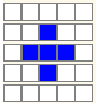
\includegraphics[scale=0.7]{fig/e_1.png} 
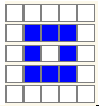
\includegraphics[scale=0.7]{fig/s_1.png} 
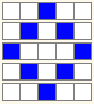
\includegraphics[scale=0.7]{fig/s_2.png} 
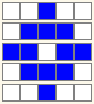
\includegraphics[scale=0.7]{fig/s_3.png} 
\end{center}

A primeira figura (da esquerda para direita) representa uma configuração inicial para o modelo, as figuras seguintes foram obtidas como resultado dos passos de evolução até alcançar a terceira geração.

Ajude Charles a simular o modelo de vida artificial citado acima.

\vspace{0.3cm}
\textbf{Entrada}

A entrada contém vários casos de teste. A primeira linha de cada caso corresponde a quantidade de gerações a ser evoluída, denominada aqui como $Q$ $(1 \leq Q \leq 100)$. A segunda linha indica a dimensão de linha $(3 \leq M \leq 100)$ e coluna $(3 \leq N \leq 100)$ da matriz bidimensional, separados por um espaço. A terceira linha possui os estados iniciais da matriz representados de forma linear (primeiro elemento, segundo elemento e assim sucessivamente), sendo o caractere $0$ o estado para células mortas e $1$ para células vivas.

O final da entrada é indicado por $Q = 0$.

\vspace{0.3cm}
\textbf{Saída}

O programa deve produzir, de forma linear, os estados de cada célula da matriz após passadas $Q$ gerações.

\begin{table}[ht]
    \centering
    \begin{tabular}{|p{7cm}|p{7cm}|}
        \hline
        \begin{center}
            \vspace{-0.3cm}
            \textbf{Exemplos de Entrada}
            \vspace{-0.3cm}
        \end{center} 
         &  
        \begin{center}
            \vspace{-0.3cm}
            \textbf{Exemplos de Saída}
            \vspace{-0.3cm}
        \end{center} \\ \hline
         \texttt{1} & \texttt{0000001110010100111000000} \\  
         \texttt{5 5} & \texttt{0010001010100010101000100} \\
         \texttt{0000000100011100010000000} & \texttt{0010001110110110111000100} \\
         \texttt{2} & \texttt{0011000000110000000000000
         0000000} \\
         \texttt{5 5} & \texttt{} \\
         \texttt{0000000100011100010000000} & \texttt{} \\
         \texttt{3} & \texttt{} \\
         \texttt{5 5} & \texttt{} \\  
         \texttt{0000000100011100010000000} & \texttt{} \\
         \texttt{7} & \texttt{} \\
         \texttt{4 8} & \texttt{} \\
         \texttt{00000000111000000010000001
         00000} & \texttt{} \\
         \texttt{0} &  \\ \hline
    \end{tabular}
    \caption{Exemplos de entradas e saídas} 
\end{table}

\newpage

\begin{center}
\noindent
\lstinputlisting{abobora_22/B/B2.cpp}
\end{center}